%---------------------------------------------------------------------------
% Content of Chapter 3 - Requirements and Use Cases
%
%---------------------------------------------------------------------------


\chapter{Requirements and Use Cases}
\label{cha:requirements}

\chabstract{
This chapter is first one focusing solely on aim of this thesis - creation of applications efficiency measuring tool. In order to actually start working on new software project, one must start from defining what actually system should do. This is exactly purpose of this chapter. First I am covering requirements analysis. Reader may find here clear definition of requirements that created system should met in less formal notation of plain English. Second section of this chapter tries to structurize those requirements into UML use cases form. 

}

%---------------------------------------------------------------------------

% System requirements subsection
%---------------------------------------------------------------------------
% System Requirements.
%
%---------------------------------------------------------------------------
 
\section{System Requirements}
\label{sec:SystemRequirements}

This section contains requirements that created system must meet. Requirements listing and description is divided into
two categories - functional and non-functional requirements. Functional requirements describes roughly what user can
do with application - it's functionality. On the other hand - nonfunctional requirements adds constraints to
functional ones, they describe conditions under which application must operate, they specify properties the software
must exhibit\cite{Windle:SoftReq}.

Requirement levels described in the following Requirements specifications using terms such as ``must'', ``must
not'', ``should/shall'' and ``should/shall not'' are to be read with reference to RFC 2119\cite{rfc:2119}.


\subsection{Functional Requirements}
\label{subsec:FunctionalRequirements}

Application should provide to end-user following functionalities:

\begin{itemize}
 \item {\bf Connect to already running JVM process using JMX extension.} 

Application should allow end user to connect to application he or she has previously started. It should be able to
connect to both remote or local process JVM. Additionally, to allow monitoring multiple processes that are running in
long distant (in terms of networking) environment, or to bypass firewall restriction, user should be able to start
remote measuring components, that aggregates result from single measurements and sends them to user in packaged manner.

 \item {\bf Aggregate monitored JVM processes into applications and clusters.}

User should be able to manage existing connections with JVMs in easy fashion, thus should be able to aggregate them
into logical units like clusters (group of nodes) or applications (collection of nodes or clusters that runs same
program)

 \item {\bf Connect to already running OCMG MainSM monitor.}

User should be able to work simultaneously with any JVM or OCM-G based application. To allow this, application must
provide facility to connect to OCMG MainSM monitor. Same requirements related to long distant environments as with JVM
applies here.

 \item {\bf Extract and list resources of given resource.}

Application should be able to visualize all resources of all resources, to which is currently connected.

 \item {\bf List properties of given resource.}

User should be able view all static metadata of given resource, like: host name, os version, JVM version, etc.

 \item {\bf List values of given resource's capabilities at current point of time.}

Per user request, application should provide value of given resource's capability (or multiple capabilities at once) at
given moment of time. 

 \item {\bf Control measuring capabilities of given resource.}

Application should provide facility to start, stop, pause and resume monitoring of given resource's capability. This
includes also definition of value gathering interval.

 \item {\bf List all capability values from given, started measurement.}

After starting measurement user should be able to view all values of given capability (in context of resource). This
includes all values since measurement was started, with on-line update in case of pending measurement.

 \item {\bf Visualize measurement results.}

User should be able to select measurement and plot results on graph. User should be able to choose at least few type of
graphs. Each graph should be able to render results from multiple measurements. Plots should be updated on-line with
capability values of pending measurements.

\end{itemize}


\subsection{Nonfunctional Requirements}
\label{subsec:NonFunctionalRequirements}


\begin{itemize}
 \item {\bf Usability.}

It is most important nonfunctional requirement - user interface should be as much user-friendly as it's possible. User
shouldn't loose his or hers time on learning how application actual works. Each function should be just in the place,
where casual user will expect it to be.

 \item {\bf Reliability.}

Application cannot have any critical bug that can cause crash. Application's failure, cannot lead to data loss.

 \item {\bf Scalability.}

User should be able to work with wide variety of environments - from single process running on single host, up to
highly distributed application running on several clusters containing vast amount of computing units.

 \item {\bf Interoperability.}

Application should operate on most currently available platforms: Linux, Windows or MacOS X.

 \item {\bf Driven by Open Source.}

To allow extend of application's life cycle, it's development should be based on open source resources.

 \item {\bf Well documented.}

Extensive documentation is crucial to allow other developers contributing to the project.

\end{itemize}




% Use Cases subsection
%---------------------------------------------------------------------------
% System use cases.
%
%---------------------------------------------------------------------------
\section{Use cases}
\label{sec:ch4_usecases}

In this section one may find a usability analysis. This analysis is divided into 3 areas covering subsequent functional blocks: resources, measurements and visualizations. For each block, diagram in UML notation with additional description is provided. This approach is equal to the second level of detail in writing use cases, as proposed by A. Cockburn\cite{0201702258}. 

Because system isn't expected to work with sensitive information, there are no authorization mechanisms or access control management considered in this work. This also implies that in all diagrams, there is only one actor: User.

\subsection{Resources Management}
\label{subsec:resources_mgmnt}

Figure \ref{fig:usecase_resources} shows diagram depicting use cases related to resources management. This includes most generic actions like adding a resource, removing a resource or viewing its state. Additionally the application enables the user to manage the life cycle of specific resources (e.g. threads, processes) - user can pause, stop or resume previously paused item. What should be also mentioned, this diagram covers indirect actions that might be performed by user, like selecting which internal monitor (the user might use more than one) should be used to manage given resource, connecting to an external monitor, or even starting it.

\begin{figure}[ht]
\centering
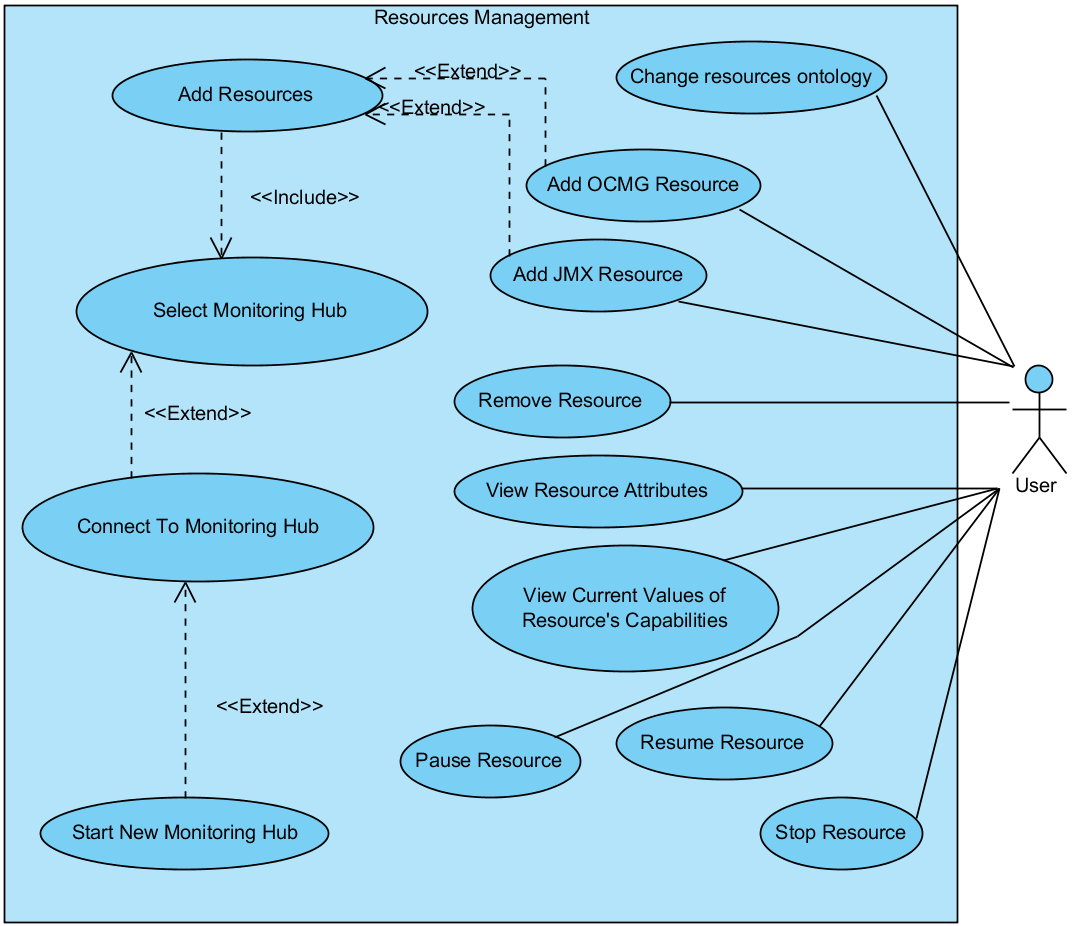
\includegraphics[width=0.8\textwidth]{resources}
\caption{Resources management use case diagram}
\label{fig:usecase_resources}
\end{figure}

The main use cases (actions performed by user directly to achieve his/hers aims) are as follows:

\begin{itemize}
\item {\bf Add an OCM-G Resource}~~~~~~~~~~~~~~~~~~~~~~~~~~~~~~~~~~~~~~~~~~~~~~~~~~~~~~~~\linebreak
Adding OCM-G resources. A OCM-G resource is a resource, monitored using the OCM-G monitoring system. This use case is a specialization of a more generic Add Resource use case. The user should be able to select application registered at the Main SM to monitor. After selecting an application, all its resources will be discovered and added to the resource tree.

\item {\bf Add a JMX Resource}~~~~~~~~~~~~~~~~~~~~~~~~~~~~~~~~~~~~~~~~~~~~~~~~~~~~~~~~\linebreak
Adding JMX resources. A JMX resource is a running JVM to which Monitoring Hub can connect using JMX protocol. While adding JMX resources, the user can arrange them into labeled clusters and applications, and must specify an URL that will be used by the monitor to connect to JVM.

\item {\bf Remove a Resource}~~~~~~~~~~~~~~~~~~~~~~~~~~~~~~~~~~~~~~~~~~~~~~~~~~~~~~~~\linebreak
Every added resource can be simply removed. All its measurements, and sub resources are removed as well.

\item {\bf View Resource Attributes} ~~~~~~~~~~~~~~~~~~~~~~~~~~~~~~~~~~~~~~~~~~~~~~~~~~~~~~~~\linebreak
By selecting a previously added resource, user should be able to view given resource's static attributes. This is highly specific to the resource type. For example, a process resource may have attributes like executable path, command line attributes, etc.

\item {\bf View Current Values of Resource's
Capabilities}~~~~~~~~~~~~~~~~~~~~~~~~~~~~~~~~~~~~~~~~~~~~~~~~~~~~~~~~\linebreak
After selecting a previously added resource, user can trigger fetching all resource\rq{}s capabilities values and thus view a snapshot of its state at a current moment of time.

\item {\bf Pause a Resource}~~~~~~~~~~~~~~~~~~~~~~~~~~~~~~~~~~~~~~~~~~~~~~~~~~~~~~~~\linebreak
User should be able to manage a resource\rq{}s life cycle, if applicable. Specific resources like threads, processes, or nodes can be paused, which freezes processing made on a given resource.

\item {\bf Resume a Resource}~~~~~~~~~~~~~~~~~~~~~~~~~~~~~~~~~~~~~~~~~~~~~~~~~~~~~~~~\linebreak
As stated above, user can pause a resource. The user should be also able to resume previously paused resource.

\item {\bf Stop a Resource}~~~~~~~~~~~~~~~~~~~~~~~~~~~~~~~~~~~~~~~~~~~~~~~~~~~~~~~~\linebreak
If a resource allows it, user should be able to stop the given resource totally. After stopping a resource, no further calculations can be performed using the given resource, and it is impossible to resume the resource again.

\item {\bf Change Resources Ontology}~~~~~~~~~~~~~~~~~~~~~~~~~~~~~~~~~~~~~~~~~~~~~~~~~~~~~~~~\linebreak
The user can change the ontology that the system internally uses to build a resources tree. This change will not  be applied to the currently discovered resource tree, but all newly added resources.

\end{itemize}


Indirect use cases (actions performed by user indirectly to help perform direct actions):

\begin{itemize}

\item {\bf Add a Resource}~~~~~~~~~~~~~~~~~~~~~~~~~~~~~~~~~~~~~~~~~~~~~~~~~~~~~~~~\linebreak
Generalization of use cases: Add JMX Resource and Add OCM-G Resource. It was extracted to ease the modeling of functionalities provided by those use cases, like selecting monitoring hub.

\item {\bf Select a Monitoring Hub}~~~~~~~~~~~~~~~~~~~~~~~~~~~~~~~~~~~~~~~~~~~~~~~~~~~~~~~~\linebreak
To be able to add a resource, the user has to select a monitor that will be responsible for managing resources and gathering data related to them.

\item {\bf Connect to a Monitor}~~~~~~~~~~~~~~~~~~~~~~~~~~~~~~~~~~~~~~~~~~~~~~~~~~~~~~~~\linebreak
User should be able, to connect to manually started, potentially remote, monitor, prior to selecting one.

\item {\bf Start a new monitor}~~~~~~~~~~~~~~~~~~~~~~~~~~~~~~~~~~~~~~~~~~~~~~~~~~~~~~~~\linebreak
User should be able to start a new, potentially remote monitoring hub, prior to connecting and using it.

\end{itemize}

\subsection{Measurements Management}
\label{subsec:measurement_mgmnt}



Figure~\ref{fig:usecases_measurements} shows the use cases related to measurement management. Measurement functionalities are a bit less complex then resources management. User is able to create and start (which is merged into one action), stop, pause, resume measuring values of given capabilities. Additionally user can view all historical values, of a given measurement.

\begin{figure}[ht]
\centering
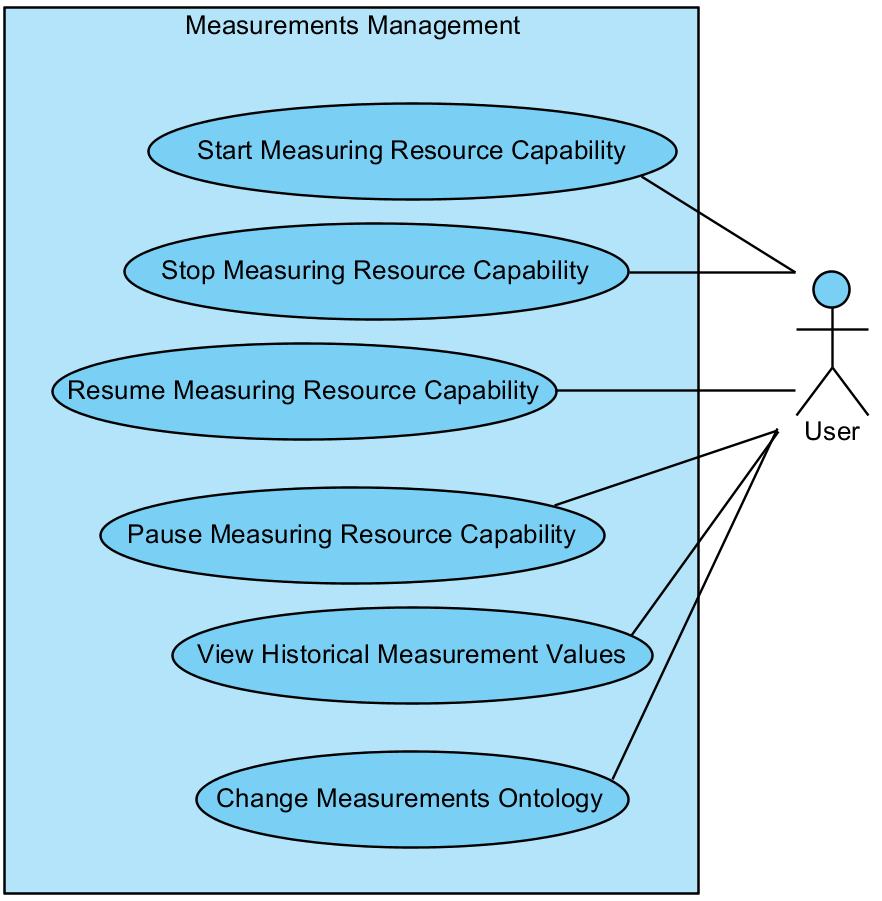
\includegraphics[width=0.5\textwidth]{Measurements}
\caption{Measurements management use case diagram}
\label{fig:usecases_measurements}
\end{figure}

\subsection{Visualizations Management}
\label{subsec:visualizations_mgmnt}

Figure~\ref{fig:usecases_visualisations} depicts the use cases related to management of measurement visualizations. The visualization functional block contains following actions:

\begin{itemize}

\item {\bf Add a visualization}~~~~~~~~~~~~~~~~~~~~~~~~~~~~~~~~~~~~~~~~~~~~~~~~~~~~~~~~\linebreak
The user can add a new, empty (without any measurements attached) visualization. It is a basic first step that needs to be done to visualize measurements.

\item {\bf Add a measurement to a visualization}~~~~~~~~~~~~~~~~~~~~~~~~~~~~~~~~~~~~~~~~~~~~~~~~~~~~~~~~\linebreak
After creating a new visualization, user can add a measurement, which makes the visualization component fully functional.

\item {\bf View a visualization}~~~~~~~~~~~~~~~~~~~~~~~~~~~~~~~~~~~~~~~~~~~~~~~~~~~~~~~~\linebreak
It is the most obvious use case - after creating a visualization and attaching a measurement the user can view results of a measurement using the provided plots.

\item {\bf Remove a measurement from a visualization}~~~~~~~~~~~~~~~~~~~~~~~~~~~~~~~~~~~~~~~~~~~~~~~~~~~~~~~~\linebreak
The user should be able to remove a previously attached measurement from a given visualization.

\item {\bf Remove a visualization}~~~~~~~~~~~~~~~~~~~~~~~~~~~~~~~~~~~~~~~~~~~~~~~~~~~~~~~~\linebreak
When the use does not need given visualization anymore, it can be simply removed.

\item {\bf Edit  visualization display options}~~~~~~~~~~~~~~~~~~~~~~~~~~~~~~~~~~~~~~~~~~~~~~~~~~~~~~~~\linebreak
The user should be able to have an additional level of control over a visualization. Management of a plot type makes it possible. The user should be able to change the display type of an already created visualization.

\item {\bf Change the measurements ontology}~~~~~~~~~~~~~~~~~~~~~~~~~~~~~~~~~~~~~~~~~~~~~~~~~~~~~~~~\linebreak
The user can change the ontology that defines capabilities that given resource has.

\end{itemize}

\begin{figure}[ht]
\centering
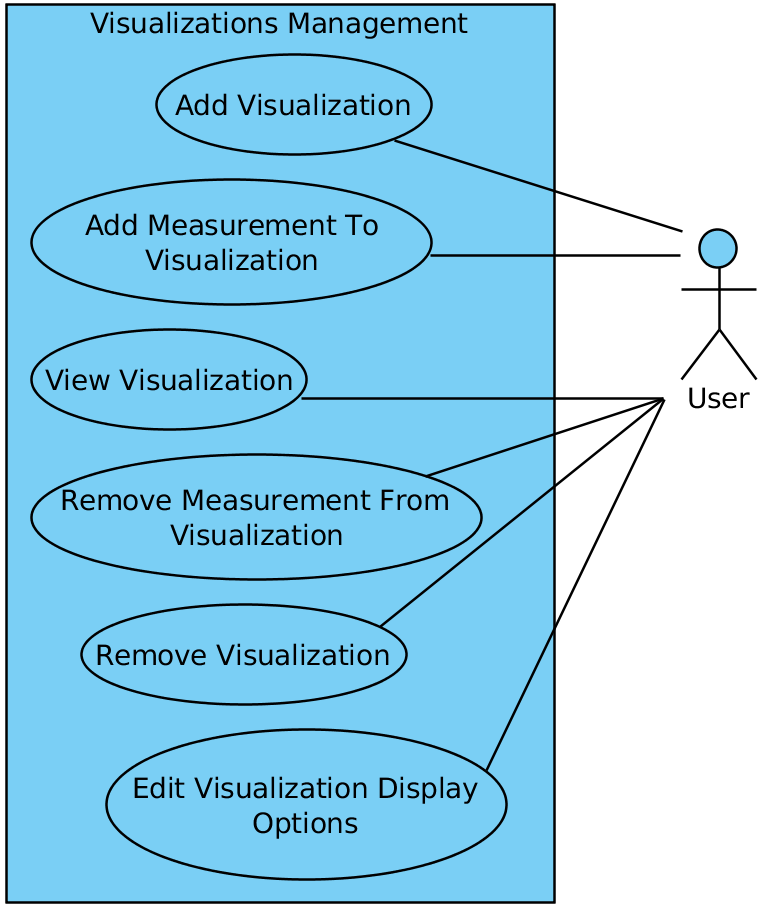
\includegraphics[width=0.4\textwidth]{Visualizations}
\caption{Use case diagram of visualizations management.}
\label{fig:usecases_visualisations}
\end{figure}







